\documentclass[10pt,a4paper,titlepage]{article}
\usepackage[utf8]{inputenc}
\usepackage{amsmath}
\usepackage{amsfonts}
\usepackage{amssymb}
\usepackage{graphicx}
\usepackage{lmodern}
\usepackage{xcolor}
\usepackage{subcaption}
\usepackage{qtree}
\usepackage{listings}
\usepackage{color}
\usepackage[xetex, hypertexnames=false, breaklinks=true, pdfborder={0 0 0},
pdfauthor={Timo Homburg},
pdftitle={Connect Four Projectdescription},
pdfsubject={Connect Four},
pdfkeywords={C,Game,Console,Connect Four},
pdfproducer={Xetex with hyperref},
pdfcreator={Pdflatex}]{hyperref}
\definecolor{gray}{rgb}{0.4,0.4,0.4}
\definecolor{darkblue}{rgb}{0.0,0.0,0.6}
\definecolor{cyan}{rgb}{0.0,0.6,0.6}
\lstset{
basicstyle=\footnotesize,
frame=single,,
  columns=fullflexible,
  showstringspaces=false,
  commentstyle=\color{gray}\upshape,
  keepspaces
                 % Linienstaerke des Rahmens
}
\lstdefinelanguage{XML}
{
  morestring=[b]",
  morestring=[s]{>}{<},
  morecomment=[s]{<?}{?>},
  stringstyle=\color{black},
  identifierstyle=\color{darkblue},
  keywordstyle=\color{cyan},
  morekeywords={xmlns,version,type}% list your attributes here
}
\begin{document}
\tableofcontents
\ \\\\\\\
\textbf{\large Connect Four Projectdescription}\\
\section{Build instructions}
To compile the program, just compile the available file using GCC or other suitable C compilers. Using a Linux shell, the commands are \begin{lstlisting}
gcc file.c -o connectfour
\end{lstlisting}
An executable "connectfour" will be created and can be started. The program can also be compiled under Windows and should not have any important operation system specific dependencies.
\section{Goal of the game}
The goal of the game for each player is to connect for stones of the same color in a diagonal, horizontal or vertical row. The player who achieves this goal first wins the game. In the event, that the gameboard is filled completely but no four stones have been connected in a diagonal, vertical or horizontal row, the game ends in a draw.
\section{Strategy of the computer opponent}
The strategy of the computer is not perfect, but developed on my own using in my first programming lecture in university. It grades the columns in which a stone can be placed with a distinct point score according to the games situation.\\
It operates as follows:
\begin{enumerate}
	\item Check (from the left of the gameboard) if a new stone can be inserted
	\item Check if in the first free column from the left there are 3 stones of the same color in a vertical, horizontal or diagonal chain. If so, this column will be graded with 120450points if the stones have the color of the computer and with 17207 points if the stones have the color of the player.
	\item  If no three stones of the same color have been found, the algorithm checks if a column left or right of the column to be checked contains more stones. If this is true, the next higher row of the column to be checked will be checkd for three same stones around it.
	If three stones of the opponents color or three stones of the computers color exist, the scoring function of step 2 is being called and its score is substracted from the first score. Subsequently it is checked if the second score is equal to the highest possible score (120450) or a multiple of it. (If this is the case the computer wins by choosing this column). If this is the case the algorithm will check for a winning situation in two rows over the current row to be checked. If there is another winning possibility, the score will be adjusted to 17206, a score under the highest score of the opponent. If the PC cannot win in this column the score will be set to -99000.
	\item In this step, step 2 will be repeated for 2 stones in horizontal, vertical and diagonal direction. The scores are set to 2458 for the opponent and 351 for the computer.
	In the special case that two opponent stones (or two own stones) in one row with two free places around them, or 2 opponent or own stones with free places around and in between them exist (socalled predicament), the score is adjusted in order to not let the opponent win in the turn after the next turn or in order to improve the chances of winning. Scores in the special cases are then set to 17207 for the opponent and 5735 for the computer.
	\item After that step 2 is repeated for a stone in horizontal, vertical and diagonal direction. The scores are 50 for the opponent player and 7 for the computer opponent. 
	\item The value from steps 2 to 5 is saved in an array of scores. The maximum value is saved in an additional variable along with its column number.
	\item If the score of a column is smaller than -99100, it will be adjusted to -99100
	\item Steps 1 to 7 will be repeated for the following 6 columns
	\item If no scores can be calculated (for example at the beginning of the game), one of the columns 3,4 or 5 will be chosen at random. Those columns are the most promising columns for a consecutive victory of the computer.
\end{enumerate}
The program includes a debug mode which can be activated using option 5 of the main menu. In this mode the scores calculated by the computer are visualized.
\section{Screenshots}
\clearpage
\begin{figure}
	\centering
	\begin{subfigure}{.5\textwidth}
		\centering
		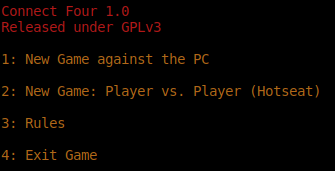
\includegraphics[width=0.9\linewidth]{img/menu.png}
		\caption{Game Menu}
		\label{fig:sub1}
	\end{subfigure}%
	\begin{subfigure}{.5\textwidth}
		\centering
		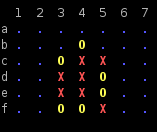
\includegraphics[width=0.9\linewidth]{img/connectfour.png}
		\caption{Game Screen}
		\label{fig:sub2}
	\end{subfigure}
	\label{fig:test}
\end{figure}
\begin{figure}
	\centering
	\begin{subfigure}{.5\textwidth}
		\centering
		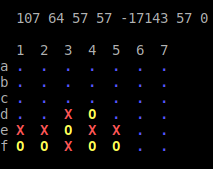
\includegraphics[width=0.9\linewidth]{img/debugmode.png}
		\caption{Debugmode}
		\label{fig:sub3}
	\end{subfigure}%
	\begin{subfigure}{.5\textwidth}
		\centering
		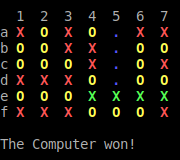
\includegraphics[width=0.9\linewidth]{img/computerwon.png}
		\caption{Computer Won}
		\label{fig:sub4}
	\end{subfigure}
	\label{fig:test}
\end{figure}
\end{document}